\documentclass{standalone}
\usepackage{tikz}
\usetikzlibrary{patterns, positioning}


\begin{document}
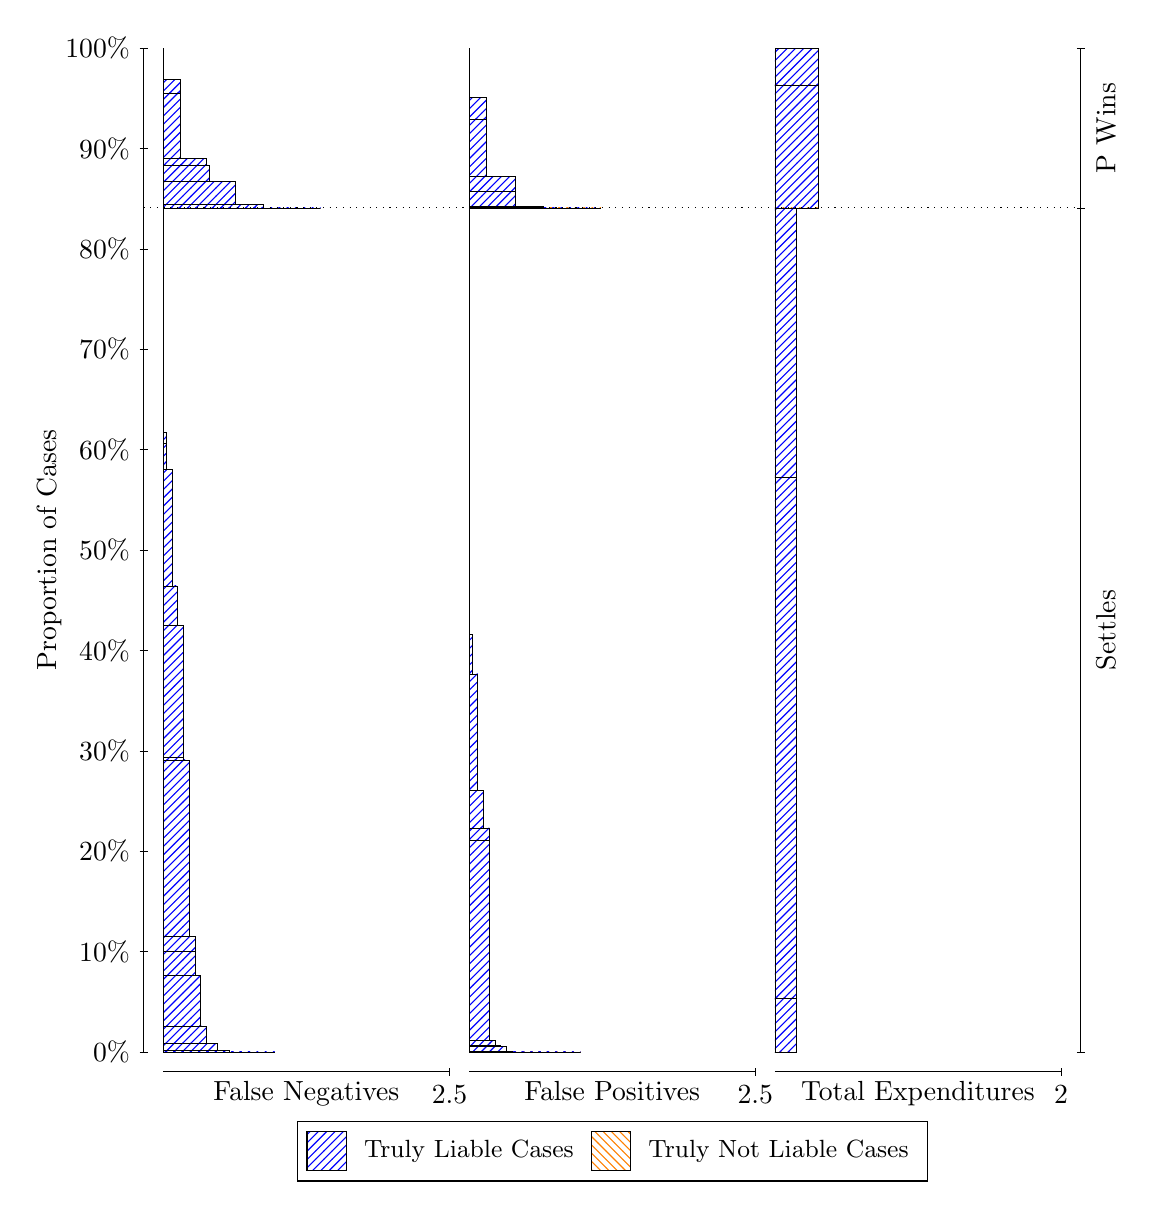
\begin{tikzpicture}
\draw[black, very thin] (1.5,1.75) -- (1.5,14.5);
\node[rotate=90, text=black, anchor=center] at (0.3, 8.125) {Proportion of Cases};
\draw[black, very thin] (1.45,1.75) -- (1.55,1.75);
\node[text=black, anchor=east] at (1.45, 1.75) {0\%};
\draw[black, very thin] (1.45,3.025) -- (1.55,3.025);
\node[text=black, anchor=east] at (1.45, 3.025) {10\%};
\draw[black, very thin] (1.45,4.3) -- (1.55,4.3);
\node[text=black, anchor=east] at (1.45, 4.3) {20\%};
\draw[black, very thin] (1.45,5.575) -- (1.55,5.575);
\node[text=black, anchor=east] at (1.45, 5.575) {30\%};
\draw[black, very thin] (1.45,6.85) -- (1.55,6.85);
\node[text=black, anchor=east] at (1.45, 6.85) {40\%};
\draw[black, very thin] (1.45,8.125) -- (1.55,8.125);
\node[text=black, anchor=east] at (1.45, 8.125) {50\%};
\draw[black, very thin] (1.45,9.4) -- (1.55,9.4);
\node[text=black, anchor=east] at (1.45, 9.4) {60\%};
\draw[black, very thin] (1.45,10.675) -- (1.55,10.675);
\node[text=black, anchor=east] at (1.45, 10.675) {70\%};
\draw[black, very thin] (1.45,11.95) -- (1.55,11.95);
\node[text=black, anchor=east] at (1.45, 11.95) {80\%};
\draw[black, very thin] (1.45,13.225) -- (1.55,13.225);
\node[text=black, anchor=east] at (1.45, 13.225) {90\%};
\draw[black, very thin] (1.45,14.5) -- (1.55,14.5);
\node[text=black, anchor=east] at (1.45, 14.5) {100\%};

\draw[black, very thin] (13.4,1.75) -- (13.4,14.5);
\draw[black, very thin] (13.35,1.75) -- (13.45,1.75);
\node[anchor=west] at (13.35, 1.75) {};
\draw[black, very thin] (13.35,12.47) -- (13.45,12.47);
\node[anchor=west] at (13.35, 12.47) {};
\draw[black, very thin] (13.35,14.5) -- (13.45,14.5);
\node[anchor=west] at (13.35, 14.5) {};

\draw[black, very thin, pattern color=blue, pattern=north east lines] (1.75,1.75) rectangle (3.167,1.75);
\draw[black, very thin, pattern color=blue, pattern=north east lines] (1.75,1.75) rectangle (2.8763,1.75);
\draw[black, very thin, pattern color=blue, pattern=north east lines] (1.75,1.75) rectangle (2.8037,1.75);
\draw[black, very thin, pattern color=blue, pattern=north east lines] (1.75,1.75) rectangle (2.731,1.75);
\draw[black, very thin, pattern color=blue, pattern=north east lines] (1.75,1.75) rectangle (2.5857,1.7731);
\draw[black, very thin, pattern color=blue, pattern=north east lines] (1.75,1.7731) rectangle (2.513,1.7748);
\draw[black, very thin, pattern color=blue, pattern=north east lines] (1.75,1.7748) rectangle (2.4403,1.8616);
\draw[black, very thin, pattern color=blue, pattern=north east lines] (1.75,1.8616) rectangle (2.3677,1.8628);
\draw[black, very thin, pattern color=blue, pattern=north east lines] (1.75,1.8628) rectangle (2.295,2.0819);
\draw[black, very thin, pattern color=blue, pattern=north east lines] (1.75,2.0819) rectangle (2.2223,2.7182);
\draw[black, very thin, pattern color=blue, pattern=north east lines] (1.75,2.7182) rectangle (2.1497,3.0262);
\draw[black, very thin, pattern color=blue, pattern=north east lines] (1.75,3.0262) rectangle (2.1497,3.2196);
\draw[black, very thin, pattern color=blue, pattern=north east lines] (1.75,3.2196) rectangle (2.077,5.459);
\draw[black, very thin, pattern color=blue, pattern=north east lines] (1.75,5.459) rectangle (2.0043,5.4908);
\draw[black, very thin, pattern color=blue, pattern=north east lines] (1.75,5.4908) rectangle (2.0043,7.1697);
\draw[black, very thin, pattern color=blue, pattern=north east lines] (1.75,7.1697) rectangle (1.9317,7.6682);
\draw[black, very thin, pattern color=blue, pattern=north east lines] (1.75,7.6682) rectangle (1.859,9.1469);
\draw[black, very thin, pattern color=blue, pattern=north east lines] (1.75,9.1469) rectangle (1.7863,9.4862);
\draw[black, very thin, pattern color=blue, pattern=north east lines] (1.75,9.4862) rectangle (1.7863,9.6235);
\draw[black, very thin, pattern color=orange, pattern=north west lines] (1.75,9.6235) rectangle (1.75,9.6235);
\draw[black, very thin, pattern color=blue, pattern=north east lines] (1.75,9.6235) rectangle (1.75,12.47);
\draw[black, very thin, pattern color=blue, pattern=north east lines] (1.75,12.47) rectangle (3.7483,12.47);
\draw[black, very thin, pattern color=blue, pattern=north east lines] (1.75,12.47) rectangle (3.385,12.47);
\draw[black, very thin, pattern color=blue, pattern=north east lines] (1.75,12.47) rectangle (3.058,12.47);
\draw[black, very thin, pattern color=blue, pattern=north east lines] (1.75,12.47) rectangle (3.0217,12.511);
\draw[black, very thin, pattern color=blue, pattern=north east lines] (1.75,12.511) rectangle (2.6947,12.511);
\draw[black, very thin, pattern color=blue, pattern=north east lines] (1.75,12.511) rectangle (2.6583,12.809);
\draw[black, very thin, pattern color=blue, pattern=north east lines] (1.75,12.809) rectangle (2.3313,13.015);
\draw[black, very thin, pattern color=blue, pattern=north east lines] (1.75,13.015) rectangle (2.295,13.095);
\draw[black, very thin, pattern color=blue, pattern=north east lines] (1.75,13.095) rectangle (1.968,13.93);
\draw[black, very thin, pattern color=blue, pattern=north east lines] (1.75,13.93) rectangle (1.968,14.103);
\draw[black, very thin, pattern color=blue, pattern=north east lines] (1.75,14.103) rectangle (1.9317,14.103);
\draw[black, very thin, pattern color=orange, pattern=north west lines] (1.75,14.103) rectangle (1.75,14.103);
\draw[black, very thin, pattern color=blue, pattern=north east lines] (1.75,14.103) rectangle (1.75,14.5);
\draw[black, very thin, pattern color=orange, pattern=north west lines] (5.6333,1.75) rectangle (7.0503,1.75);
\draw[black, very thin, pattern color=blue, pattern=north east lines] (5.6333,1.75) rectangle (7.0503,1.75);
\draw[black, very thin, pattern color=orange, pattern=north west lines] (5.6333,1.75) rectangle (6.905,1.75);
\draw[black, very thin, pattern color=blue, pattern=north east lines] (5.6333,1.75) rectangle (6.905,1.75);
\draw[black, very thin, pattern color=orange, pattern=north west lines] (5.6333,1.75) rectangle (6.7597,1.75);
\draw[black, very thin, pattern color=blue, pattern=north east lines] (5.6333,1.75) rectangle (6.7597,1.75);
\draw[black, very thin, pattern color=blue, pattern=north east lines] (5.6333,1.75) rectangle (6.687,1.75);
\draw[black, very thin, pattern color=orange, pattern=north west lines] (5.6333,1.75) rectangle (6.6143,1.75);
\draw[black, very thin, pattern color=blue, pattern=north east lines] (5.6333,1.75) rectangle (6.6143,1.75);
\draw[black, very thin, pattern color=blue, pattern=north east lines] (5.6333,1.75) rectangle (6.5417,1.75);
\draw[black, very thin, pattern color=orange, pattern=north west lines] (5.6333,1.75) rectangle (6.469,1.75);
\draw[black, very thin, pattern color=blue, pattern=north east lines] (5.6333,1.75) rectangle (6.469,1.75);
\draw[black, very thin, pattern color=blue, pattern=north east lines] (5.6333,1.75) rectangle (6.3963,1.75);
\draw[black, very thin, pattern color=orange, pattern=north west lines] (5.6333,1.75) rectangle (6.3237,1.75);
\draw[black, very thin, pattern color=blue, pattern=north east lines] (5.6333,1.75) rectangle (6.3237,1.75);
\draw[black, very thin, pattern color=blue, pattern=north east lines] (5.6333,1.75) rectangle (6.251,1.7503);
\draw[black, very thin, pattern color=orange, pattern=north west lines] (5.6333,1.7503) rectangle (6.1783,1.7503);
\draw[black, very thin, pattern color=blue, pattern=north east lines] (5.6333,1.7503) rectangle (6.1783,1.7546);
\draw[black, very thin, pattern color=blue, pattern=north east lines] (5.6333,1.7546) rectangle (6.1057,1.8185);
\draw[black, very thin, pattern color=blue, pattern=north east lines] (5.6333,1.8185) rectangle (6.033,1.8369);
\draw[black, very thin, pattern color=blue, pattern=north east lines] (5.6333,1.8369) rectangle (5.9603,1.9016);
\draw[black, very thin, pattern color=orange, pattern=north west lines] (5.6333,1.9016) rectangle (5.8877,1.9016);
\draw[black, very thin, pattern color=blue, pattern=north east lines] (5.6333,1.9016) rectangle (5.8877,4.4434);
\draw[black, very thin, pattern color=blue, pattern=north east lines] (5.6333,4.4434) rectangle (5.8877,4.5961);
\draw[black, very thin, pattern color=blue, pattern=north east lines] (5.6333,4.5961) rectangle (5.815,5.0727);
\draw[black, very thin, pattern color=blue, pattern=north east lines] (5.6333,5.0727) rectangle (5.7423,6.5514);
\draw[black, very thin, pattern color=blue, pattern=north east lines] (5.6333,6.5514) rectangle (5.6697,7.0499);
\draw[black, very thin, pattern color=blue, pattern=north east lines] (5.6333,7.0499) rectangle (5.6333,12.47);
\draw[black, very thin, pattern color=orange, pattern=north west lines] (5.6333,12.47) rectangle (7.3047,12.47);
\draw[black, very thin, pattern color=blue, pattern=north east lines] (5.6333,12.47) rectangle (7.3047,12.47);
\draw[black, very thin, pattern color=orange, pattern=north west lines] (5.6333,12.47) rectangle (6.9413,12.47);
\draw[black, very thin, pattern color=blue, pattern=north east lines] (5.6333,12.47) rectangle (6.9413,12.47);
\draw[black, very thin, pattern color=blue, pattern=north east lines] (5.6333,12.47) rectangle (6.9413,12.47);
\draw[black, very thin, pattern color=orange, pattern=north west lines] (5.6333,12.47) rectangle (6.578,12.47);
\draw[black, very thin, pattern color=blue, pattern=north east lines] (5.6333,12.47) rectangle (6.578,12.478);
\draw[black, very thin, pattern color=blue, pattern=north east lines] (5.6333,12.478) rectangle (6.578,12.489);
\draw[black, very thin, pattern color=orange, pattern=north west lines] (5.6333,12.489) rectangle (6.251,12.489);
\draw[black, very thin, pattern color=blue, pattern=north east lines] (5.6333,12.489) rectangle (6.251,12.489);
\draw[black, very thin, pattern color=orange, pattern=north west lines] (5.6333,12.489) rectangle (6.2147,12.489);
\draw[black, very thin, pattern color=blue, pattern=north east lines] (5.6333,12.489) rectangle (6.2147,12.684);
\draw[black, very thin, pattern color=blue, pattern=north east lines] (5.6333,12.684) rectangle (6.2147,12.867);
\draw[black, very thin, pattern color=blue, pattern=north east lines] (5.6333,12.867) rectangle (5.8877,12.867);
\draw[black, very thin, pattern color=orange, pattern=north west lines] (5.6333,12.867) rectangle (5.8877,12.867);
\draw[black, very thin, pattern color=blue, pattern=north east lines] (5.6333,12.867) rectangle (5.8877,12.867);
\draw[black, very thin, pattern color=blue, pattern=north east lines] (5.6333,12.867) rectangle (5.8513,13.601);
\draw[black, very thin, pattern color=blue, pattern=north east lines] (5.6333,13.601) rectangle (5.8513,13.875);
\draw[black, very thin, pattern color=orange, pattern=north west lines] (5.6333,13.875) rectangle (5.6333,13.875);
\draw[black, very thin, pattern color=blue, pattern=north east lines] (5.6333,13.875) rectangle (5.6333,14.5);
\draw[black, very thin, pattern color=orange, pattern=north west lines] (9.5167,1.75) rectangle (9.7892,1.75);
\draw[black, very thin, pattern color=blue, pattern=north east lines] (9.5167,1.75) rectangle (9.7892,2.4376);
\draw[black, very thin, pattern color=orange, pattern=north west lines] (9.5167,2.4376) rectangle (9.7892,2.4376);
\draw[black, very thin, pattern color=blue, pattern=north east lines] (9.5167,2.4376) rectangle (9.7892,9.0496);
\draw[black, very thin, pattern color=orange, pattern=north west lines] (9.5167,9.0496) rectangle (9.7892,9.0496);
\draw[black, very thin, pattern color=blue, pattern=north east lines] (9.5167,9.0496) rectangle (9.7892,12.47);
\draw[black, very thin, pattern color=orange, pattern=north west lines] (9.5167,12.47) rectangle (10.062,12.47);
\draw[black, very thin, pattern color=blue, pattern=north east lines] (9.5167,12.47) rectangle (10.062,14.033);
\draw[black, very thin, pattern color=orange, pattern=north west lines] (9.5167,14.033) rectangle (10.062,14.033);
\draw[black, very thin, pattern color=blue, pattern=north east lines] (9.5167,14.033) rectangle (10.062,14.5);
\draw[black, dotted] (1.5,12.47) -- (13.4,12.47);
\draw[black, very thin] (1.75,1.5) -- (5.3833,1.5);
\node[text=black, anchor=north] at (3.5667, 1.5) {False Negatives};
\draw[black, very thin] (5.3833,1.45) -- (5.3833,1.55);
\node[text=black, anchor=north] at (5.3833, 1.45) {2.5};

\draw[black, very thin] (5.6333,1.5) -- (9.2667,1.5);
\node[text=black, anchor=north] at (7.45, 1.5) {False Positives};
\draw[black, very thin] (9.2667,1.45) -- (9.2667,1.55);
\node[text=black, anchor=north] at (9.2667, 1.45) {2.5};

\draw[black, very thin] (9.5167,1.5) -- (13.15,1.5);
\node[text=black, anchor=north] at (11.333, 1.5) {Total Expenditures};
\draw[black, very thin] (13.15,1.45) -- (13.15,1.55);
\node[text=black, anchor=north] at (13.15, 1.45) {2};

\node[text=black, centered, rotate=90] at (13.72, 7.1098) {Settles};
\node[text=black, centered, rotate=90] at (13.72, 13.485) {P Wins};

\draw (7.449999999999999,1.5) node[draw=none] (baseCoordinate) {};
\begin{scope}[align=center]
        \matrix[scale=0.5, draw=black, below=0.5cm of baseCoordinate, nodes={draw}, column sep=0.1cm]{
            \node[rectangle, draw, minimum width=0.5cm, minimum height=0.5cm, pattern color=blue, pattern=north east lines] {}; &
            \node[draw=none, font=\small, text=black] (B) {Truly Liable Cases}; &
            \node[rectangle, draw, minimum width=0.5cm, minimum height=0.5cm, pattern color=orange, pattern=north west lines] {}; &
            \node[draw=none, font=\small, text=black] (B) {Truly Not Liable Cases}; \\
            };
\end{scope}

\end{tikzpicture}
\end{document}